\documentclass[12 pt]{amsart}
\usepackage{amsmath, amssymb, amsthm,amscd}
\usepackage{tkz-graph}
\usepackage{tikz}
\usepackage{tikz,fullpage}
\usetikzlibrary{positioning, quotes}
\usetikzlibrary{arrows,%
                petri,%
                topaths}%
\usetikzlibrary{graphs,quotes}
\usetikzlibrary{arrows,automata}
\usepackage[latin1]{inputenc}
\usepackage{tkz-berge}
\usepackage[position=top]{subfig}

\allowdisplaybreaks

\newcommand{\mathsym}[1]{{}}
\newcommand{\unicode}{{}}

\newtheorem{theorem}{Theorem}[section]
\newtheorem{lemma}[theorem]{Lemma}
\newtheorem{proposition}[theorem]{Proposition}
\newtheorem{corollary}[theorem]{Corollary}
\newtheorem{definition}[theorem]{Definition}
\newtheorem{construction}[theorem]{Construction}

\newcommand\T{\rule{0pt}{4.0ex}}       % Top strut
\newcommand\B{\rule[-2.5ex]{0pt}{0pt}} % Bottom strut

\newcommand{\smat}[4] {(\begin{smallmatrix} #1 & #2 \\ #3 & #4 \end{smallmatrix} )}
\newcommand{\mat}[4]  { \left(\begin{array}{cc} #1 & #2 \\ #3 & #4 \end{array} \right)}
\newcommand{\schar}[2] {( \begin{smallmatrix} #1 \\ #2 \end{smallmatrix})}

\newcommand{\op}[1]  { \operatorname{ #1 }}
\newcommand{\olbbH}[0]  { \overline{\mathbb{H}}}
\newcommand{\olbbQ}[0]  { \overline{\mathbb{Q}}}
\newcommand{\olG}[0]  { \overline{\Gamma}}
\newcommand{\bbH}[0]  { \mathbb{H}}
\newcommand{\bbC}[0]  { \mathbb{C}}
\newcommand{\bbZ}[0]  { \mathbb{Z}}
\newcommand{\bbF}[0]  { \mathbb{F}}
\newcommand{\bbQ}[0]  { \mathbb{Q}}
\newcommand{\bbR}[0]  { \mathbb{R}}
\newcommand{\gok}[0]  { \mathfrak{k}}
\newcommand{\goe}[0]  { \mathfrak{e}}
\newcommand{\goR}[0]  { \mathfrak{R}}

\addtolength{\textwidth}{0.0in}
\addtolength{\hoffset}{-0.0in}
\addtolength{\textheight}{0.0in}
\addtolength{\voffset}{-0.0in}

\begin{document}
\title{matching mathematica patterns}
\author{Daniel Schultz}
\begin{abstract}
A process to construct machines recognizing mathematica patterns is discussed. This makes the pattern matching process completely transparent, and we attempt to either match some of the behaviour exhibited by WRI's implementation or improve on it.
\end{abstract}
\maketitle

\section{Introduction}
\subsection{orderless} When matching {\tt f[a,b,c,d,e]} against {\tt f[x\_\_,y\_\_]} with an orderless {\tt f}, one will find that WRI's matcher does not even consider the possibility {\tt x=b,a}, {\tt y=c,d,e}. This is apparently because {\tt b,a} is itself out of order and the pattern matcher does not change the order in sequences. While not completely ideal, we reproduce this behaviour simply because it cuts down on the number of possiblity to be tried while still retaining some useful functionality: $2^5$ is much smaller than $5!$.
\subsection{flat} When matching {\tt f[a,b,a,b,c,d,e]} against {\tt f[(x\_)..,y\_\_,z\_\_]}, we allow {\tt x} to match {\tt f[a,b]}.

\section{Architecture of the compiler}
Besides the pattern that is to be constructed, the function for converting a pattern to a machine takes the following arguments:
\begin{itemize}
\item A stack of symbols called {\tt vars} which consists of the variables currently being recorded (from {\tt Pattern}). If the the symbol $x$ is uninitialized, the instruction $start(x)$ will at run time cause the instruction $capture(x)$ to append the local variable $cur$ to $x$. The instruction $stop(x)$ will stop such appends and put the symbol $x$ in the initialized state. If the symbol $x$ is initialized, the instruction $start(x)$ will at run time cause the instruction $capture(x)$ to start comparing with the currently stored sequence for $x$. Then, the instruction $stop(x)$ will check that the number of expressions checked by the captures matches the original number of values captured in the initial $start(x)$ - $stop(x)$ pair.
\item A stack of expressions called {\tt tests}. The instruction $test(f)$ will apply $f$ to the value of the local variable $cur$ and fail if the return is not exactly {\tt True}. This is used to implement {\tt PaternTest}.
\item A boole {\tt ishead} indicating if we are in the head of a pattern.
\item A boole {\tt isFlat} indicating if we are in the arguments of a flat head.
\item A boole {\tt isOrderless} indicating if we are in the arguments of an orderless head.
\end{itemize}

We have the following runtime local variables of the pattern matcher machine:
\begin{itemize}
\item An integer $i$ which starts at $i=0$. This is the index of the current child we are looking at ($i=0$ correspondes to the head).
\item An expression $cur$ which is the most recent child looked at in the current subexpression.
\end{itemize}
The instructions $down$ (resp. $up$) are responsible for moving $down$ from parent to child (resp. up from child to parent) and constructing a new stack frame for $i$ and $cur$ (resp. destroying it) These are all operation done at runtime when the pattern matcher is trying to match, and not done in the process of compiling a pattern. The most important routine with respect to the variables $i$ and $cur$ is the $next$ routine, which is responsible for choosing a new argument from the arguments of the expressions passed to the matcher.

\section{basic routines}
\subsection{bootstrapping}
To compile the pattern $p$ at the top level we use
\begin{center}
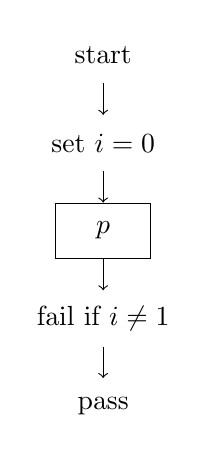
\begin{tikzpicture}[
     node distance = 4mm and 4mm,
every label/.style = {label distance=3pt, fill=white, inner sep=1pt},
        box/.style = {rectangle, minimum width=12mm, minimum height=7mm},
        dbox/.style = {rectangle, draw, minimum width=12mm, minimum height=7mm}
                        ]
\node (start)[box] {start};
\node (first)  [box,below  =of start] {set $i = 0$};
\node (p) [dbox,below  =of first] {$p$};
\node (check)  [box,below  =of p] {fail if $i\ne 1$};
\node (pass)  [box,below =of check] {pass};
\draw[->] (start) to (first);
\draw[->] (first) to (p);
\draw[->] (p) to (check);
\draw[->] (check) to (pass);
\end{tikzpicture}
\end{center}
The box around $p$ means that it should be compiled recursively according to the rules given below and its $start$ and $end$ nodes should be spliced in. $p$ should be compiled with {\tt vars} and {\tt tests} both empty and {\tt ishead=True}. This bootstrapping step is a little awkward because it means that the final pattern matcher must be passed $e[]$ when matching $e$. However, this is the simplest way to ensure that {\tt BlankSequence} and {\tt BlankNullSequence} do not get erroneously matched at the top level.

\subsection{Routine for patternless expressions} If $p$ is a pattern free from expressions related to pattern matching, it may be compiled as
\begin{center}
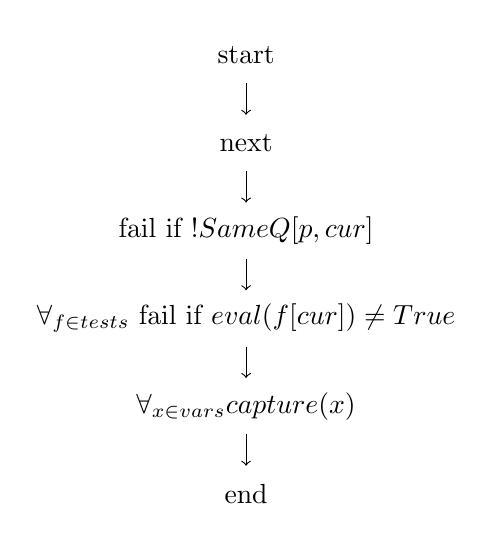
\begin{tikzpicture}[
     node distance = 4mm and 4mm,
every label/.style = {label distance=3pt, fill=white, inner sep=1pt},
        box/.style = {rectangle, minimum width=12mm, minimum height=7mm},
        dbox/.style = {rectangle, draw, minimum width=12mm, minimum                        height=7mm}
                        ]
\node (start)[box] {start};
\node (next)  [box,below  =of start] {next};
\node (cmp) [box,below  =of next] {fail if $!SameQ[p, cur]$};
\node (test)  [box,below  =of cmp] {$\forall_{f \in tests}$ fail if $eval(f[cur]) \neq True$};
\node (cap)  [box,below  =of test] {$\forall_{x \in vars} capture(x)$};
\node (end)[box, below =of cap] {end};
\draw[->] (start) to (next);
\draw[->] (next) to (cmp);
\draw[->] (cmp) to (test);
\draw[->] (test) to (cap);
\draw[->] (cap) to (end);
\end{tikzpicture}
\end{center}
The routine $next$ depends on the context supplied by the context in \ref{subsection_node} and is described in Section \ref{subsection_next}.

\subsection{Routine for nodes without pattern-related heads}
\label{subsection_node}
The pattern $p_0[p_1, \dots, p_n]$ where $p_0$ has no meaning related to patterns (basically it's not in Section \ref{section_pheads}) may be compiled as
\begin{center}
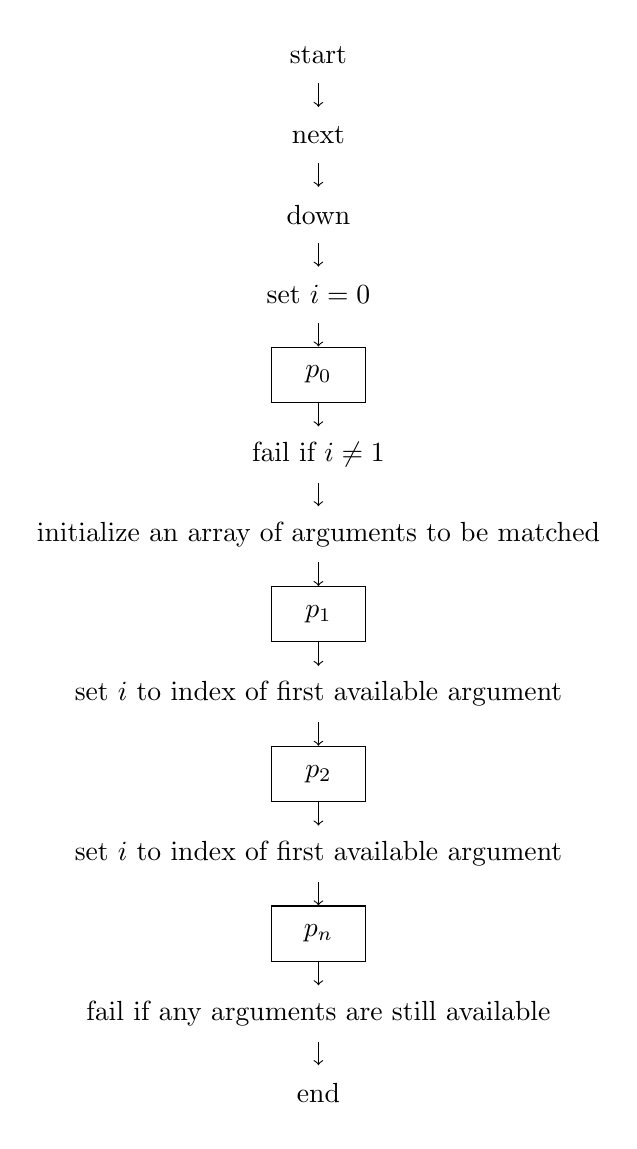
\begin{tikzpicture}[
     node distance = 3mm and 3mm,
every label/.style = {label distance=3pt, fill=white, inner sep=1pt},
        box/.style = {rectangle, minimum width=12mm, minimum height=7mm},
        dbox/.style = {rectangle, draw, minimum width=12mm, minimum                        height=7mm}
                        ]
\node (start)[box] {start};
\node (next)  [box,below  =of start] {next};
\node (down) [box,below  =of next] {down};
\node (starthead) [box,below  =of down] {set $i=0$};
\node (e0) [dbox,below  =of starthead] {$p_0$};
\node (endhead) [box,below  =of e0] {fail if $i \ne 1$};
\node (init) [box,below  =of endhead] {initialize an array of arguments to be matched};
\node (e1) [dbox,below  =of init] {$p_1$};
\node (e2i) [box,below  =of e1] {set $i$ to index of first available argument};
\node (e2) [dbox,below  =of e2i] {$p_2$};
\node (eni) [box,below  =of e2] {set $i$ to index of first available argument};
\node (en) [dbox,below  =of eni] {$p_n$};
\node (endchild) [box,below  =of en] {fail if any arguments are still available};
\node (end)[box, below =of endchild] {end};
\draw[->] (start) to (next);
\draw[->] (next) to (down);
\draw[->] (down) to (starthead);
\draw[->] (starthead) to (e0);
\draw[->] (e0) to (endhead);
\draw[->] (endhead) to (init);
\draw[->] (init) to (e1);
\draw[->] (e1) to (e2i);
\draw[->] (e2i) to (e2);
\draw[->] (e2) to (eni);
\draw[->] (eni) to (en);
\draw[->] (en) to (endchild);
\draw[->] (endchild) to (end);
\end{tikzpicture}
\end{center}
All of the $p_i$ should be compiled with empty {\tt vars} and empty {\tt tests}. $p_0$ should be compiled with {\tt ishead=True} and $p_1, \dots, p_n$ should be compiled with {\tt ishead=False} and {\tt isFlat}, {\tt isOrderless} set according to $p_0$. The instruction ``initialize an array of arguments to be matched'' needs to mark each of the children of the expression $e$ to be matched as available. When the instruction $next$ in Section \ref{subsection_next} consumes a child via $e_{i++}$ this child of index $i$ needs be marked as unavailable. When there are no more available children, the instruction ``set $i$ to index of first available argument'' should set $i$ to an integer greater than the length of the expression to be matched. This will ensure that all calls to $i++$ or $e_{i++}$ fail.

\subsection{Routine $next$ for heads and childs}
\label{subsection_next}
Incrementing $i$ when it is already past the length of the expression $e$ to be matched should be considered a fail. In all of these routines, the increment on $i$ ($i++$) will be a simple ``add one'' when the corresponding head is not orderless. However, when the head is orderless, it should move $i$ to the next available child. Similarly, $e_{i++}$ should mark the $i$th child as unavailable before incrementing $i$.
The following one routine is for head mode ({\tt ishead=True}). The values of {\tt isFlat} and {\tt isOrderless} do not matter in this case.
Routine $next$ with {\tt ishead=True}:
\begin{center}
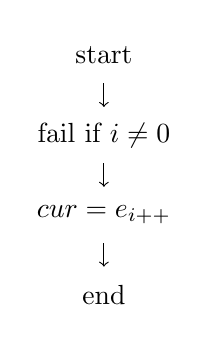
\begin{tikzpicture}[
     node distance = 3mm and 3mm,
every label/.style = {label distance=3pt, fill=white, inner sep=1pt},
        box/.style = {rectangle, draw=none, fill=#1,
                     minimum width=12mm, minimum height=7mm}
                        ]
\node (start) [box=white] {start};
\node (fail) [box=white,below  =of start] {fail if $i \ne 0$};
\node (inc) [box=white,below  =of fail] {$cur=e_{i++}$};
\node (end) [box=white,below =of inc] {end};
\draw[->] (start) to (fail);
\draw[->] (fail) to (inc);
\draw[->] (inc) to (end);
\end{tikzpicture}
\end{center}

The following are all for child mode ({\tt ishead=False}). Routine $next$ with {\tt isFlat=False} and {\tt Orderless=False}:
\begin{center}
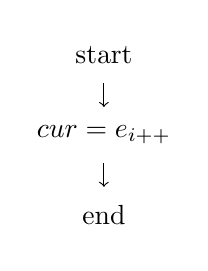
\begin{tikzpicture}[
     node distance = 3mm and 3mm,
every label/.style = {label distance=3pt, fill=white, inner sep=1pt},
        box/.style = {rectangle, draw=none, fill=#1,
                     minimum width=12mm, minimum height=7mm}
                        ]
\node (start) [box=white] {start};
\node (inc) [box=white,below  =of start] {$cur=e_{i++}$};
\node (end) [box=white,below =of inc] {end};
\draw[->] (start) to (inc);
\draw[->] (inc) to (end);
\end{tikzpicture}
\end{center}

Routine $next$ with {\tt isFlat=False} and {\tt isOrderless=True}:
\begin{center}
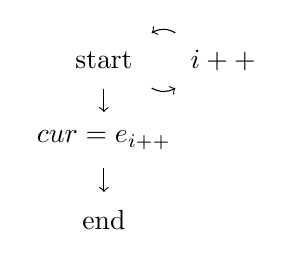
\begin{tikzpicture}[
     node distance = 3mm and 3mm,
every label/.style = {label distance=3pt, fill=white, inner sep=1pt},
        box/.style = {rectangle, draw=none, fill=#1,
                     minimum width=12mm, minimum height=7mm}
                        ]
\node (start) [box=white] {start};
\node (skip) [box=white,right  =of start] {$i++$};
\node (inc) [box=white,below  =of start] {$cur=e_{i++}$};
\node (end) [box=white,below =of inc] {end};
\draw[->] (start) to (inc);
\draw[->] (inc) to (end);
\draw[->] (start)[bend right] to (skip);
\draw[->] (skip)[bend right] to (start);
\end{tikzpicture}
\end{center}

Routine $next$ with {\tt isFlat=True} (head $f$) and {\tt isOrderless=False}:
\begin{center}
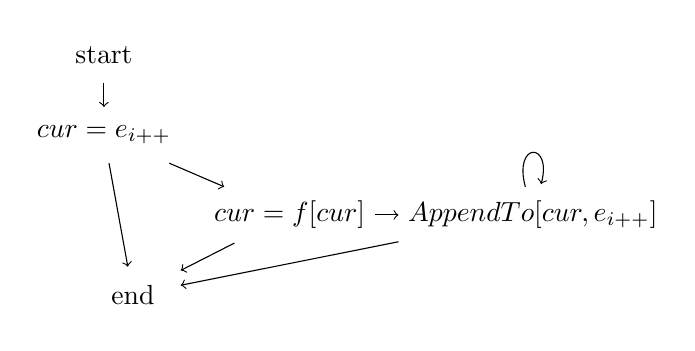
\begin{tikzpicture}[
     node distance = 3mm and 3mm,
every label/.style = {label distance=3pt, fill=white, inner sep=1pt},
        box/.style = {rectangle, draw=none, fill=#1,
                     minimum width=12mm, minimum height=7mm}
                        ]
\node (start) [box=white] {start};
\node (inc) [box=white,below  =of start] {$cur=e_{i++}$};
\node (flat) [box=white,below right  =of inc] {$cur=f[cur]$};
\node (end) [box=white,below left =of flat] {end};
\node (append) [box=white,right =of flat] {$AppendTo[cur,e_{i++}]$};
\draw[->] (start) to (inc);
\draw[->] (inc) to (end);
\draw[->] (inc) to (flat);
\draw[->] (flat) to (end);
\draw[->] (flat) to (append);
\draw[->] (append) to (end);
\draw (append) edge[loop above] (append);
\end{tikzpicture}
\end{center}

Routine $next$ with {\tt isFlat=True} (head $f$) and {\tt isOrderless=True}:
\begin{center}
\begin{tikzpicture}[
     node distance = 3mm and 3mm,
every label/.style = {label distance=3pt, fill=white, inner sep=1pt},
        box/.style = {rectangle, draw=none, fill=#1,
                     minimum width=12mm, minimum height=7mm}
                        ]
\node (start) [box=white] {start};
\node (skip1) [box=white,right  =of start] {$i++$};
\node (inc) [box=white,below  =of start] {$cur=e_{i++}$};
\node (flat) [box=white,below right  =of inc] {$cur=f[cur]$};
\node (end) [box=white,below left =of flat] {end};
\node (null) [box=white,right =of flat] {$.$};
\node (skip2) [box=white,above  =of null] {$i++$};
\node (append) [box=white,right =of null] {$AppendTo[cur,e_{i++}]$};
\draw[->] (start)[bend right] to (skip);
\draw[->] (skip)[bend right] to (start);
\draw[->] (start) to (inc);
\draw[->] (inc) to (end);
\draw[->] (inc) to (flat);
\draw[->] (flat) to (end);
\draw[->] (flat) to (null);
\draw[->] (null) to (append);
\draw[->] (null)[bend right] to (skip2);
\draw[->] (skip2)[bend right] to (null);
\draw[->] (null) to (end);
\draw[->] (append)[bend left] to (null);
\end{tikzpicture}
\end{center}

Note that WRI's implementation only gives $next$ such a special behaviour with respect to {\tt Flat} when it is in a {\tt Blank[]} at the top level of a child (possibliy only having a {\tt Pattern} object as a parent).
\section{pattern heads}
\label{section_pheads}
\subsection{{\tt Blank}}
$Blank[]$ may be compiled as
\begin{center}
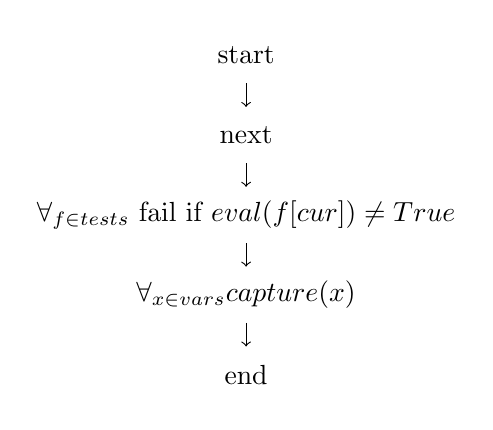
\begin{tikzpicture}[
     node distance = 3mm and 3mm,
every label/.style = {label distance=3pt, fill=white, inner sep=1pt},
        box/.style = {rectangle, minimum width=12mm, minimum height=7mm},
        dbox/.style = {rectangle, draw, minimum width=12mm, minimum                        height=7mm}
                        ]
\node (start)[box] {start};
\node (next)  [box,below  =of start] {next};
\node (test)  [box,below  =of next] {$\forall_{f \in tests}$ fail if $eval(f[cur]) \neq True$};
\node (cap)  [box,below  =of test] {$\forall_{x \in vars} capture(x)$};
\node (end)[box, below =of cap] {end};
\draw[->] (start) to (next);
\draw[->] (next) to (test);
\draw[->] (test) to (cap);
\draw[->] (cap) to (end);
\end{tikzpicture}
\end{center}
$Blank[h]$ may be compiled by inserting an instruction testing the head of $cur$ after the $next$ instruction.


\subsection{{\tt BlankSequence}}
$BlankSequence[]$ may be compiled as
\begin{center}
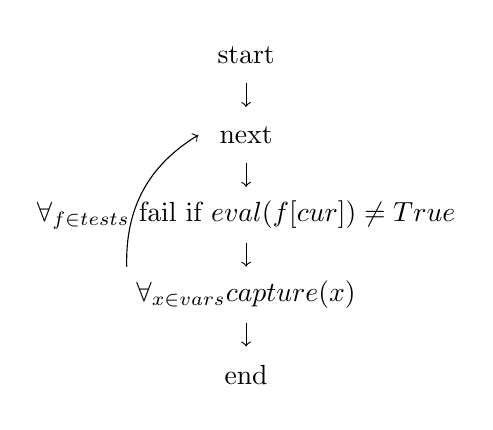
\begin{tikzpicture}[
     node distance = 3mm and 3mm,
every label/.style = {label distance=3pt, fill=white, inner sep=1pt},
        box/.style = {rectangle, minimum width=12mm, minimum height=7mm},
        dbox/.style = {rectangle, draw, minimum width=12mm, minimum                        height=7mm}
                        ]
\node (start)[box] {start};
\node (next)  [box,below  =of start] {next};
\node (test)  [box,below  =of next] {$\forall_{f \in tests}$ fail if $eval(f[cur]) \neq True$};
\node (cap)  [box,below  =of test] {$\forall_{x \in vars} capture(x)$};
\node (end)[box, below =of cap] {end};
\draw[->] (start) to (next);
\draw[->] (next) to (test);
\draw[->] (test) to (cap);
\draw[->] (cap) to (end);
\draw[->] (cap.north west)[bend left] to (next.west);
\end{tikzpicture}
\end{center}
The $next$ routine here should ignore the {\tt isFlat} flag, i.e. set it to false.
\subsection{{\tt BlankNullSequence}}
$BlankNullSequence[]$ may be compiled as
\begin{center}
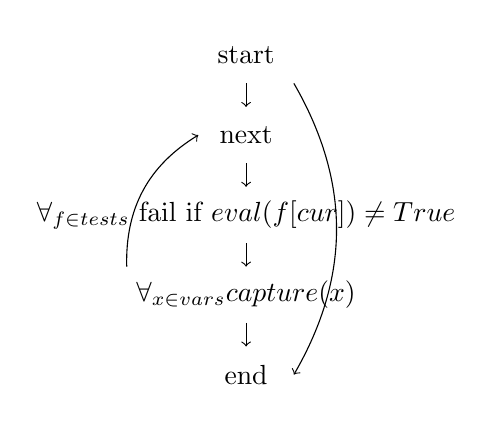
\begin{tikzpicture}[
     node distance = 3mm and 3mm,
every label/.style = {label distance=3pt, fill=white, inner sep=1pt},
        box/.style = {rectangle, minimum width=12mm, minimum height=7mm},
        dbox/.style = {rectangle, draw, minimum width=12mm, minimum                        height=7mm}
                        ]
\node (start)[box] {start};
\node (next)  [box,below  =of start] {next};
\node (test)  [box,below  =of next] {$\forall_{f \in tests}$ fail if $eval(f[cur]) \neq True$};
\node (cap)  [box,below  =of test] {$\forall_{x \in vars} capture(x)$};
\node (end)[box, below =of cap] {end};
\draw[->] (start) to (next);
\draw[->] (next) to (test);
\draw[->] (test) to (cap);
\draw[->] (cap) to (end);
\draw[->] (cap.north west)[bend left] to (next.west);
\draw[->] (start.south east)[bend left] to (end.east);
\end{tikzpicture}
\end{center}
The $next$ routine here should ignore the {\tt isFlat} flag, i.e. set it to false.

\subsection{{\tt Pattern}}
$Pattern[s,p]$ for a symbol $s$ may be compiled as
\begin{center}
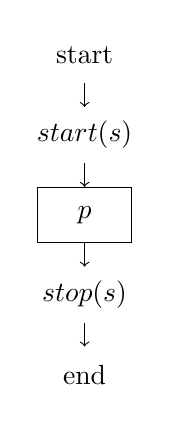
\begin{tikzpicture}[
     node distance = 3mm and 3mm,
every label/.style = {label distance=3pt, fill=white, inner sep=1pt},
        box/.style = {rectangle, minimum width=12mm, minimum height=7mm},
        dbox/.style = {rectangle, draw, minimum width=12mm, minimum                        height=7mm}
                        ]
\node (start)[box] {start};
\node (startx)  [box,below  =of start] {$start(s)$};
\node (p)  [dbox,below  =of startx] {$p$};
\node (stopx)  [box,below  =of p] {$stop(s)$};
\node (end)[box, below =of stopx] {end};
\draw[->] (start) to (startx);
\draw[->] (startx) to (p);
\draw[->] (p) to (stopx);
\draw[->] (stopx) to (end);
\end{tikzpicture}
\end{center}
Before $p$ is compiled, $s$ should be pushed onto {\tt vars}. Then, $p$ should be compiled with parameters matching those of the calling environment. After $s$ is compiled, {\tt vars} should be popped.
\subsection{{\tt PatternTest}}
$PatternTest[p,f]$ may be compiled as
\begin{center}
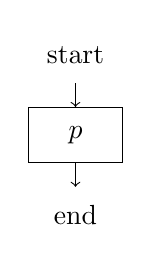
\begin{tikzpicture}[
     node distance = 3mm and 3mm,
every label/.style = {label distance=3pt, fill=white, inner sep=1pt},
        box/.style = {rectangle, minimum width=12mm, minimum height=7mm},
        dbox/.style = {rectangle, draw, minimum width=12mm, minimum                        height=7mm}
                        ]
\node (start)[box] {start};
\node (p)  [dbox,below  =of start] {$p$};
\node (end)[box, below =of p] {end};
\draw[->] (start) to (p);
\draw[->] (p) to (end);
\end{tikzpicture}
\end{center}
Before $p$ is compiled, $f$ should be pushed onto {\tt tests}. Then, $p$ should be compiled with parameters matching those of the calling environment. After $p$ is compiled, {\tt tests} should be popped.

\subsection{{\tt PatternSequence}}
$PatternSequence[p_1,\dots,p_n]$ may be compiled as
\begin{center}
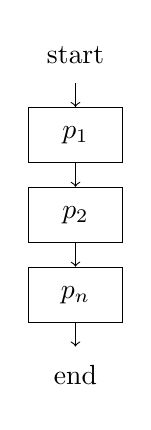
\begin{tikzpicture}[
     node distance = 3mm and 3mm,
every label/.style = {label distance=3pt, fill=white, inner sep=1pt},
        box/.style = {rectangle, minimum width=12mm, minimum height=7mm},
        dbox/.style = {rectangle, draw, minimum width=12mm, minimum                        height=7mm}
                        ]
\node (start)[box] {start};
\node (p1)  [dbox,below  =of start] {$p_1$};
\node (p2)  [dbox,below  =of p1] {$p_2$};
\node (pn)  [dbox,below  =of p2] {$p_n$};
\node (end)[box, below =of pn] {end};
\draw[->] (start) to (p1);
\draw[->] (p1) to (p2);
\draw[->] (p2) to (pn);
\draw[->] (pn) to (end);
\end{tikzpicture}
\end{center}
All $p_i$ should be compiled with parameters matching those of the calling environment.

\subsection{{\tt Alternatives}}
$Alternatives[p_1,\dots,p_n]$ may be compiled as
\begin{center}
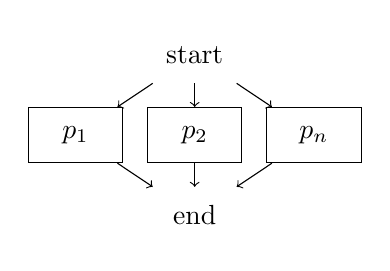
\begin{tikzpicture}[
     node distance = 3mm and 3mm,
every label/.style = {label distance=3pt, fill=white, inner sep=1pt},
        box/.style = {rectangle, minimum width=12mm, minimum height=7mm},
        dbox/.style = {rectangle, draw, minimum width=12mm, minimum                        height=7mm}
                        ]
\node (start)[box] {start};
\node (p2)  [dbox,below  =of start] {$p_2$};
\node (p1)  [dbox,left  =of p2] {$p_1$};
\node (pn)  [dbox,right  =of p2] {$p_n$};
\node (end)[box, below =of p2] {end};
\draw[->] (start) to (p1);
\draw[->] (p1) to (end);
\draw[->] (start) to (p2);
\draw[->] (p2) to (end);
\draw[->] (start) to (pn);
\draw[->] (pn) to (end);
\end{tikzpicture}
\end{center}
All $p_i$ should be compiled with parameters matching those of the calling environment.

\subsection{{\tt Repeated}}
$Repeated[p]$ may be compiled as
\begin{center}
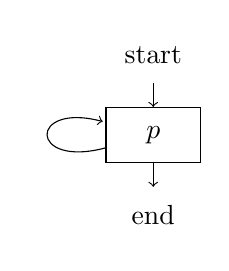
\begin{tikzpicture}[
     node distance = 3mm and 3mm,
every label/.style = {label distance=3pt, fill=white, inner sep=1pt},
        box/.style = {rectangle, minimum width=12mm, minimum height=7mm},
        dbox/.style = {rectangle, draw, minimum width=12mm, minimum                        height=7mm}
                        ]
\node (start)[box] {start};
\node (p)  [dbox,below  =of start] {$p$};
\node (end)[box, below =of p] {end};
\draw[->] (start) to (p);
\draw[->] (p) to (end);
\draw (p) edge[loop left] (p);
\end{tikzpicture}
\end{center}
$p$ should be compiled with parameters matching those of the calling environment.

\subsection{{\tt RepeatedNull}}
$RepeatedNull[p]$ may be compiled as
\begin{center}
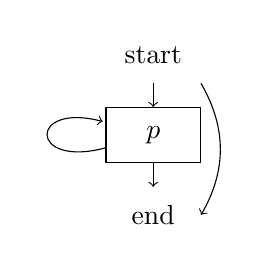
\begin{tikzpicture}[
     node distance = 3mm and 3mm,
every label/.style = {label distance=3pt, fill=white, inner sep=1pt},
        box/.style = {rectangle, minimum width=12mm, minimum height=7mm},
        dbox/.style = {rectangle, draw, minimum width=12mm, minimum                        height=7mm}
                        ]
\node (start)[box] {start};
\node (p)  [dbox,below  =of start] {$p$};
\node (end)[box, below =of p] {end};
\draw[->] (start) to (p);
\draw[->] (p) to (end);
\draw (p) edge[loop left] (p);
\draw[->] (start.south east)[bend left] to (end.east);
\end{tikzpicture}
\end{center}
$p$ should be compiled with parameters matching those of the calling environment.

\subsection{{\tt Condition}}
$Condition[p, f]$ may be compiled as
\begin{center}
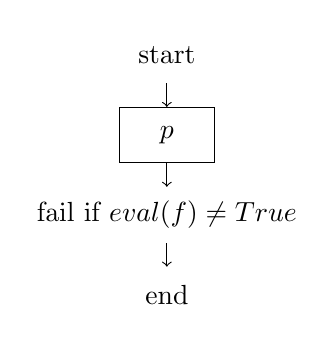
\begin{tikzpicture}[
     node distance = 3mm and 3mm,
every label/.style = {label distance=3pt, fill=white, inner sep=1pt},
        box/.style = {rectangle, minimum width=12mm, minimum height=7mm},
        dbox/.style = {rectangle, draw, minimum width=12mm, minimum                        height=7mm}
                        ]
\node (start)[box] {start};
\node (p)  [dbox,below  =of start] {$p$};
\node (f)  [box,below  =of p] {fail if $eval(f) \neq True$};
\node (end)[box, below =of f] {end};
\draw[->] (start) to (p);
\draw[->] (p) to (f);
\draw[->] (f) to (end);
\end{tikzpicture}
\end{center}
$p$ should be compiled with parameters matching those of the calling environment.

\subsection{{\tt Optional}}
$Optional[Pattern[s,p],v]$ for a symbol $s$ may be compiled as
\begin{center}
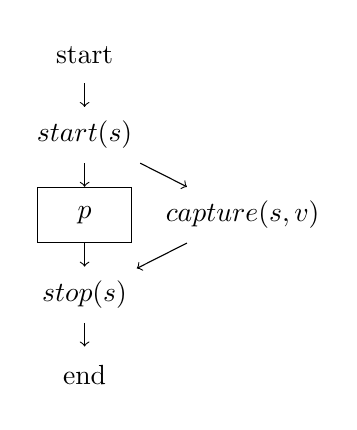
\begin{tikzpicture}[
     node distance = 3mm and 3mm,
every label/.style = {label distance=3pt, fill=white, inner sep=1pt},
        box/.style = {rectangle, minimum width=12mm, minimum height=7mm},
        dbox/.style = {rectangle, draw, minimum width=12mm, minimum                        height=7mm}
                        ]
\node (start)[box] {start};
\node (startx)  [box,below  =of start] {$start(s)$};
\node (p)  [dbox,below  =of startx] {$p$};
\node (cap)  [box,right  =of p] {$capture(s, v)$};
\node (stopx)[box, below =of p] {$stop(s)$};
\node (end)[box, below =of stopx] {end};
\draw[->] (start) to (startx);
\draw[->] (startx) to (p);
\draw[->] (p) to (stopx);
\draw[->] (stopx) to (end);
\draw[->] (startx) to (cap);
\draw[->] (cap) to (stopx);
\end{tikzpicture}
\end{center}
Of course {\tt vars} should be pushed with $s$ and popped around the compilation of $p$. The special two argument form of $capture$ captures into $s$ not the value of $cur$ but the constant value $v$.

TODO: see if this matches WRI implementation, in particular, do the {\tt tests} from $PatternTest$ affect the capture of $v$?

\section{implementation issues}



It seems very possible to match mathematica patterns by machine. Many nodes in the resulting machine have more than one outgoing path: the pattern is said to match if there is some path from the $start$ node (of the bootstrapping step) to the $pass$ node without hitting a $fail$. In practice this need to be implemented via backtracking by saving the state every time a decision is made.

\subsection{substitution of captures}
There is an issue of how the captured variables should be substituted into expressions when they require evaluation (for example, in {\tt Condition}). It seems reasonable to leave an uninitialized variable as itself and splice in initialized variables. It seems that WRI's implementation sometimes treats uninitialized variables as {\tt Sequence[]}.

\subsection{side effects}
If the main evaluations implied by {\tt Condition} or {\tt PatternTest} involve computation with side effects, we should consider the behaviour of the pattern matcher to be undefined, especially if these side effects include changing the attributes of the heads involved in matching!

\subsection{Repeated[BlankNullSequence[]]}
The savvy reader will have noticed that {\tt x\_\_\_..} results in a machine with an infinite loop. Such infinite loops only result from the back edges of {\tt Repeated} and {\tt RepeatedNull}, and this problem can be resolved by failing if the value of $i$ is the same as it was the last time the back edge was taken.

\end{document}
\grid
\grid
